%
%  assignment
%
%  Created by Matteo Casenove on 2012-09-10.
%  Copyright (c) 2012 . All rights reserved.
%
\documentclass[]{article}

% Use utf-8 encoding for foreign characters
\usepackage[utf8]{inputenc}

% Setup for fullpage use
\usepackage{fullpage}

% Uncomment some of the following if you use the features
%
% Running Headers and footers
%\usepackage{fancyhdr}

% Multipart figures
%\usepackage{subfigure}

% More symbols
%\usepackage{amsmath}
%\usepackage{amssymb}
%\usepackage{latexsym}

% Surround parts of graphics with box
\usepackage{boxedminipage}

% Package for including code in the document
\usepackage{listings}
\usepackage{color}
\usepackage{float}


\definecolor{dkgreen}{rgb}{0,0.6,0}
\definecolor{gray}{rgb}{0.5,0.5,0.5}
\definecolor{mauve}{rgb}{0.58,0,0.82}

\lstset{frame=tb,
  language=Java,
  aboveskip=3mm,
  belowskip=3mm,
  showstringspaces=false,
  columns=flexible,
  basicstyle={\small\ttfamily},
  numbers=none,
  numberstyle=\tiny\color{gray},
  keywordstyle=\color{blue},
  commentstyle=\color{dkgreen},
  stringstyle=\color{mauve},
  breaklines=true,
  breakatwhitespace=true
  tabsize=3
}

\usepackage{tikz}
\usetikzlibrary{calc,shapes.multipart,chains,arrows}

% If you want to generate a toc for each chapter (use with book)
%\usepackage{minitoc}

% This is now the recommended way for checking for PDFLaTeX:
\usepackage{ifpdf}

%\newif\ifpdf
%\ifx\pdfoutput\undefined
%\pdffalse % we are not running PDFLaTeX
%\else
%\pdfoutput=1 % we are running PDFLaTeX
%\pdftrue
%\fi


\title{1st Assignment Concurrency and Multithreading}
\author{Matteo Casenove (mce470, S2517141), Nicola Mularoni(nmi520, s2523003)}

\date{\today}

\begin{document}

%\ifpdf
%\DeclareGraphicsExtensions{.pdf, .jpg, .tif}
%\else
%\DeclareGraphicsExtensions{.eps, .jpg}
%\fi

\maketitle

%\let\clearpage\relax

\section{CoarseGrainedList}
\label{coarsegrainedlist}

\begin{figure}[H]
	\centering
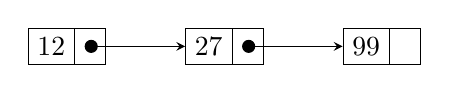
\begin{tikzpicture}[list/.style={rectangle split, rectangle split parts=2,
    draw, rectangle split horizontal}, >=stealth, start chain]

  \node[list,on chain] (A) {12};
  \node[list,on chain] (B) {27};
  \node[list,on chain] (C) {99};
  %\node[on chain,draw,inner sep=6pt] (D) {};
  %\draw (D.north east) -- (D.south west);
  %\draw (D.north west) -- (D.south east);
  \draw[*->] let \p1 = (A.two), \p2 = (A.center) in (\x1,\y2) -- (B);
  \draw[*->] let \p1 = (B.two), \p2 = (B.center) in (\x1,\y2) -- (C);
  %\draw[*->] let \p1 = (C.two), \p2 = (C.center) in (\x1,\y2) -- (D);
\end{tikzpicture}
	\caption{Example of list}
	\label{fig:list}
\end{figure}

This structure represent a really basic list structure. Each element of the list is a pair (Value, Next). It permits to insert double elements in the same list. When a new element is added to the list it must be placed right after the last element lesser or equal at it.\newline

The requirements define that the whole list has to be blocked in order to make any changes (add, remove). This means that we need only one lock for all the structure. In order to do that the code can use the simple java Lock. When a method modifies the list, it will acquire this lock until it finishes the updating of the list. The other threads have to wait until the previous thread releases it in order to acquire the lock and then update the list. This is valid also for the \emph{toString} method that prints all the structure.\newline


An element of the list can be represented as following:\newline

\begin{lstlisting}
	class Element<T>{
		T value;
		Element<T> next;
	}
\end{lstlisting}

As well as the next ones, the element implements the \emph{Comparable$<$T$>$} interface in order to sort the element in the list. This requires to implement the method \emph{compareTo} using the generic type T.

The \emph{toString} method will produce the following output for the list represented in figure \ref{fig:list}:\newline

\begin{lstlisting}
	[12][27][99]
\end{lstlisting}


The performance of this kind of list is $\mathcal{O}(N)$, where $N$ is the number of elements in the list. To add a new element to the list, the method must go through to the whole list doing at most $N$ steps.\newline


Unfortunately the coarse-grained locking significantly reduce opportunity for parallelism so, using only one lock for the whole structure it is not possible to scale it. Even using more threads working at the same structure, only one of them can work on it at a time since the lock is unique for the all structure. There is no increasing of performances using multiple threads.








\section{CoarseGrainedTree}
\label{coarsegrainedtree}


\begin{figure}[H]
	\centering
	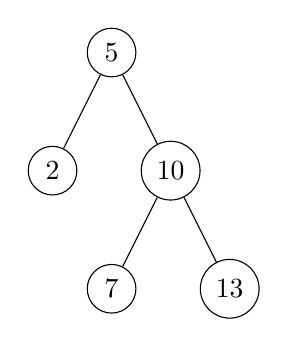
\begin{tikzpicture}
	    \tikzstyle{every node}=[circle,draw]
	    \node {5}
	        child { node {2} }
	        child {
	            node {10}
	            child { node {7} }
	            child { node {13} }
	        }
	    ;
	\end{tikzpicture}
	\caption{Example of binary search tree}
	\label{fig:tree}
\end{figure}

A Binary Search Tree (BST) is another basic structure as the list. It is represented with nodes and leafs. Each node is composed by a value and two pointers which link to its subtrees.


Considering the value of a generic node as V, every node on its right subtree contains a value greater than V, and on its left subtree all the values are lesser or equal at V. \newline


The insertion of a new element in the tree starts from the root and goes to the right or left subtree according to the value of the current node, until reaching the leaf. When a new element is already present in the tree, its is added as a new left child node of the first occurrence of the equal element. If the node already have a left child this will become the left child of the new node.


Removing an element from the tree consist of removing the first occurrence of the element and it will be replaced with one of the two children subtree.\newline


The \emph{toString} method will produce the following output for the tree represented in figure \ref{fig:tree}:\newline

\begin{lstlisting}
	[5[2][10[7][13]]]
\end{lstlisting}

According to the requirements, all the tree must be locked during the updating procedures so it will need only one lock for the whole structure. As in the CoarseGrainedList, we can use the simple java Lock.

Unfortunately, using only one lock the structure is not scalable and with multiple threads only one  can work on it at time. This means that as well as the previous structure, there is no gain in performance with multiple threads.


The performance of the tree for a generic update is $\mathcal{O}(\log N)$, where $N$ is the number of nodes and $\log N$ is the depth of the tree.\newline

The structure of node can be represented as following:\newline

\begin{lstlisting}
	class Node<T>{
		T value;
		Node<T> left;
		Node<T> right;
	}
\end{lstlisting}



\section{FineGrainedList}
\label{finegrainedlist}
%\node[list,on chain,style={draw=blue!50}] (A) {12};


Fine Grained List has the same structure of the one described in section \ref{coarsegrainedlist}. The only difference now is that it does not require the lock for the whole structure anymore. This relaxation in the requirements permits to have one lock for each element of the list permitting then to work in different parts of the list at the same time. 


On the other hand, this increases the complexity of the checks in order to maintain the consistency of the structure.\newline

%The requirements define that the whole list has to be blocked in order to make any changes (add, remove). This means that we need only one lock for all the structure. In order to do that the code can use the simple java Lock. When a method modifies the list, it will acquire this lock until it finishes the updating of the list. The other threads have to wait until the previous thread releases it in order to acquire the lock and then update the list.\newline


The new element of the list can be represented as following:\newline

\begin{lstlisting}
	class Element<T>{
		boolean marked;
		Lock lock;
		T value;
		Element<T> next;
	}
\end{lstlisting}

Using multiple locks makes difference in the \emph{add} and \emph{remove} methods. In order to \emph{add} or \emph{remove} an element in the list, the methods have to find the correct position in the list and select the two element: predecessor and current. Then they have to lock these two elements and eventually make the changes. Instead, the method \emph{toString} needs only to lock the current element. In this way it will print the status of the structure at the moment it is moving through the structure. Of course this will not be the real status of the whole structure because in the meanwhile it is printing one part, another thread could remove an element that the \emph{toString} already printed.\newline


As described in the book, section 9.7, between the research of the element and the lock of the element another thread can modify the list, even removing the element already found. For this reason it is introduced a \emph{validation} method to check the status of the locked elements. This resolves the concurrency problem between multiple threads working on the same part of the list. The status consists of a flag that marks an element when it is removed. This is called logic remove.\newline

The pseudo code for the generic update method will be as the following:\newline

\begin{lstlisting}
	update(T value){
		if searchElementInTheList is true then{
			select the predecessor and current element
		}
			return false
		lock predecessor 
		lock current
		if validation is true then{
			update procedure
			unlock current
			unlock predecessor
			return true
		}else
			unlock current
			unlock predecessor
			return update(value)
	}
\end{lstlisting}

The update procedure consist of adding or removing an element from the list. If the validation fails the update method restarts from the beginning.


It is also important to notice that the order of the locks has an important meaning for the concurrency. All the threads have to lock the elements with the same order: first the \emph{predecessor} and then the \emph{current} element. If it is not so, deadlocks can occur. Moreover, the order of the updates of the links is important, for example to add a new element: first update the new element link to \emph{current}, and then update the \emph{predecessor} to the new element. This order avoids to break the chain and that if another thread goes through the list during an updating procedure it will not occur find a cul-de-sac.


The double elements are managed as described in the section \ref{coarsegrainedlist} for the Coarse Grained List.\newline


Locking only two elements of the list, all the others are free and others threads can modify them without being stopped by the first one. This means that if we have a sufficiently big number of elements all the threads can pretty much work at the same time. This is a big step forward for the performances compare to the Coarse Grained List. If the number of elements is not sufficiently big for the number of threads, of course the performances return close to the ones of the previous kind of list. The threads will be stopped by the locks of the others. 

Moreover, the lock itself require time. Using a lot of locks, we have a lot of communication with the kernel and each time the bus at hardware level has to be locked and released. This produce overhead.








\section{FineGrainedTree}
\label{finegrainedtree}

This kind of structure is basically the same discussed in \ref{coarsegrainedtree}; the main difference between theese two structures, is the use of the locks.

Putting a lock for each node of the tree means to complicate the management of the whole structure in favor of the possibility to work concurrently on the tree for more than one thread and reduces lock contention.
\newline 

Like in the FineGrainedList structure, described in \ref{finegrainedlist}, we need to add to each node a Boolean marked field indicating whether that node is in the set; by doing this, we avoid problems like the attempt of a thread to add a node as a child of a node that another thread wants to remove.
\newline

Taking in account what discussed above, the new element of the tree can be represented as following:\newline

\begin{lstlisting}
	class Node<T>{
		boolean marked;
		Lock lock;
		T value;
		Node<T> left;
		Node<T> right;
	}
\end{lstlisting}

For the same reasons discussed in \ref{finegrainedlist} we need a \emph{validation} method that has to check the actual status of the lock elements.
\newline

To add a new element in the tree, a thread must acquire the lock on the node that will become the parent of the new node.
If the new element is already present in the tree and if the node with the same value already has a left child, the thread must acquire the lock on both nodes.
\newline

The \emph{remove} method has to acquire the right number of locks (depending on the position of the node), from the parent of the target node until is needed;
than the method has to mark the target node, logically removing it, and than redirects all the pointers needed as in a standard BST delection, physically removing the node.

It is important also in this case that all the locks must be acquired in the same order from all the thread, otherwise the deadlock is inevitable.

By doing this, the method has to acquire a number of locks between 2 (the best case in which the target node is a leaf) and $\log d$ where d is the depth of the first left leaf in the right subtree (or viceversa).

\begin{figure}
	\centering
	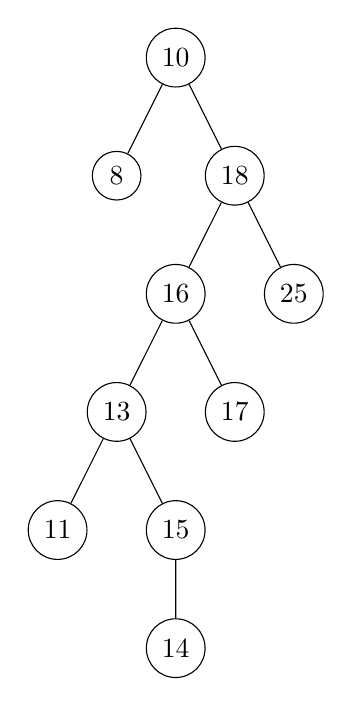
\begin{tikzpicture}
	    \tikzstyle{every node}=[circle,draw]
	    \node {10}
	        child { node {8} }
	        child {
	            node {18}
	            child { 
	            		node {16}
	            		child{
	            			node{13}
	            			child{ node{11} }
	            			child{ 
	            				node{15}
	            				child{ node{14} }
	            			}
	            		}
	            		child{ node {17} }
	            	}
	            child { node {25} }
	        }
	    ;
	\end{tikzpicture}
	\caption{Example of the worst case}
	\label{fig:badTree}
\end{figure}

Obviously this kind of use of the locks, leads to a degradation of the performance (especially if the structure is not well populated with respect to the number of threads).
\newline

There are some kinds of fix like marking the node that has been deleted as rooted, without phisically removing it, but then we will need also a method for checking if a rooted node can be phisically removed (sooner or later should be removed) and also a method to rebalance the tree in case it becomes too unbalanced.

As discussed in \ref{finegrainedlist}, the method \emph{toString} has to acquire the lock only on the current node (if it not marked) but also in this case, the structure that will be printed could be not the real status of it but only a partial one, since it can be modified meanwhile.
The order in which the node are printed is the same described in \ref{coarsegrainedtree}.
\newline

However the performance with respect to CoarseGrainedTree are improved in terms of concurrency, but the methods are still not wait-free.

\section{LockFreeList}
\label{lockfreelist}

To implement a non-blocking structure, we need atomic \emph{read-modify-write} primitives that the hardware must provide; the paragraph 9.8 of the book shows how \emph{compareAndSet} can be used in combination with the \emph{AtomicMarkableReference<T>}  (provided by \textbf{java.util.concurrent.atomic} ) that in our case incapsulate both a reference to an object of type T and the Boolean mark introduced in \ref{finegrainedlist} and in \ref{finegrainedtree} producing an atomical update of both of them.
\newline

By doing this we ensure that a node's fields cannot be updated after that node has been logically or physically removed from the list. 

The new element of the list can be represented as following:\newline

\begin{lstlisting}
	class Element<T>{
		boolean marked;
		Lock lock;
		T value;
		AtomicMarkableReference<Element<T>> next;
	}
\end{lstlisting}

We also need that each thread that want to perform an add or a remove operation, while traverses the list, cleans up the list by physically removing any marked nodes it encounters.

The main differences between the structure we are asked to implement and the one described in book are the use of the interface Comparable and the presence of duplicated keys.

The first difference mainly affects the comparison between the nodes that are made through the method \emph{compareTo} provided by the interface;
the second difference is dealt like in \ref{coarsegrainedlist} and in \ref{finegrainedlist}.

The method \emph{toString} needs to check if the node is marked or not through the method \emph{isMarked} provided by the \emph{AtomicMarkableReference} class before printing it; the only problem that could arise is if between the result of isMarked and the actual print of the node another thread mark the node as logically deleted but like in the other structure discussed above, this method prints an image of the structure as it appears while the method is traversing it.

The introduction of atomic modification of a reference and a Boolean mark causes an overhead that impacts on the performance and also the fact that both \emph{add} and \emph{remove} could engage in concurrent cleanup of removed nodes introduces the possibility of contention among threads.

\section{LockFreeTree}

In the paper \cite{nonblock} is described a design and an implementation of the Non-Blocking Binary Search Tree. This is the same structure we have to follow and use to implement our Lock Free Tree. At this point we do not have the restriction of using double element anymore, the only difference in our case is that the internal node implementation.\newline

The paper introduces also two new structures \emph{DInfo} and \emph{IInfo}. The first one contains the information necessary to remove a node; the second contains the information for the insertion of a new value in the tree. These two structures are introduced in order to permit other threads to help the updating procedure. They also extend the class Info.\newline

The IInfo structure can be represented as follow:\newline

\begin{lstlisting}
	class IInfo extend Info{
		Node p;
		Node l;
		Node newInternal;
	}
\end{lstlisting}

The DInfo structure can be represented as follow:\newline

\begin{lstlisting}
	class DInfo extend Info{
		Node gp;
		Node p;
		Node l;
		StateInfo si;
	}
\end{lstlisting}

These two structures are created when an add or a remove operation is performed. The StateInfo structure represents the couple of values state and info that are stored in the internal node. In the internal node the state contains the flag that specify in which state it is during an update operation. The info contains the link to either an IInfo object or a DInfo object, where all the information for the update operation are stored. The StateInfo object in DInfo is a copy of the old value of the StateInfo object of the internal node.\newline

The StateInfo structure can be represented as follow:\newline

\begin{lstlisting}
	class StateInfo{
		String state;
		Info info;	
	}
\end{lstlisting}

At this point the internal node has the following structure:\newline

\begin{lstlisting}
	class Internal<T> extend Node{
		AtomicReference<StateInfo> si;
		T value;
		Node<T> left;
		Node<T> right;	
	}
\end{lstlisting}

As we can see, the node contains an \emph{AtomicReference} object. It is the object that permits to use the \emph{compareAndSet} method for the atomic operation. It has \emph{StateInfo} as generic type in order to make the updating procedure of the values of \emph{state} and \emph{info} a single atomic operation.

The leaf contains only the value and it extends the type \emph{Node} as well as the internal node.\newline

Another big difference from the paper is that we have the \emph{toString} method that print the structure. We assume that, as the other methods  this one also helps to update the structure. It does not print the value of the leaf until the status of the internal node that it has reached is \emph{CLEAN}. In this way, there are no consistency problems of the printed structure.\newline

All the concurrency problems are solved by the algorithm proposed in the paper so we do not have to add additional structure to solve them. 


The performances of this structure are the best we can reach. It is fully scaled and every thread that competes for an update helps to resolve the status that could make it wait. In this way none of them actually wait without doing anything but every one works to resolve the problem. Of course, having a bigger number of thread compare to the number of node does not help much because they will do the same work. 

In this case, we do not have overhead produced by the locks because all the work is performed by the atomic method \emph{compareAndSet}.













%\begin{abstract}
%\end{abstract}

%\section{Introduction}

%\bibliographystyle{plain}
%\bibliography{}

\begin{thebibliography}{9}

\bibitem{nonblock}
  Faith Ellen, Panagiota Fatourou
  \emph{Non-blocking Binary Search Trees}.
  2010.

\end{thebibliography}

\end{document}
